\subsection{Pixel size, magnification and resolution}
Our result from calculating how many pixels in the image (see figure \ref{fig:TestChart}) that corresponds to one centimetre were 41. When we calculated the length of a car in the image (see figure \ref{fig:Toy1}) we got the result 10 cm. When comparing the resolution from two images of a object at different distances, we got the result of more pixels per cm when closer to the object.

\begin{figure}[h]
	\centering
	\begin{subfigure}[b]{0.3\textwidth}
		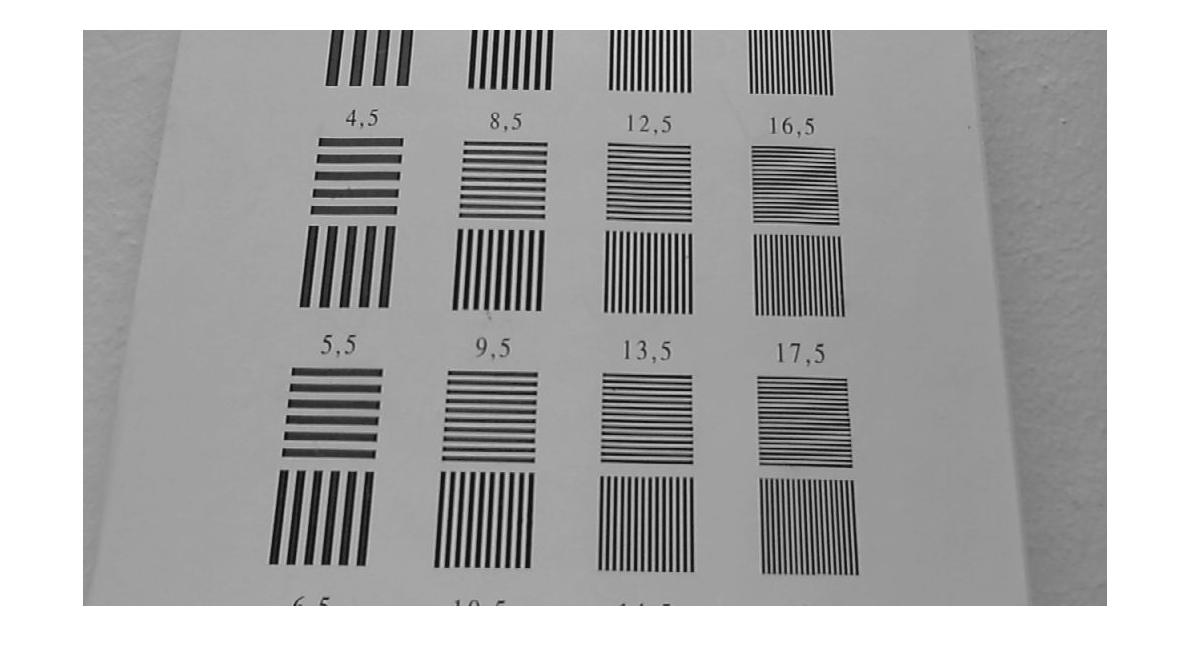
\includegraphics[width=\textwidth]{part1image1}
		\caption{}
		\label{fig:TestChart}
	\end{subfigure}
	\begin{subfigure}[b]{0.3\textwidth}
		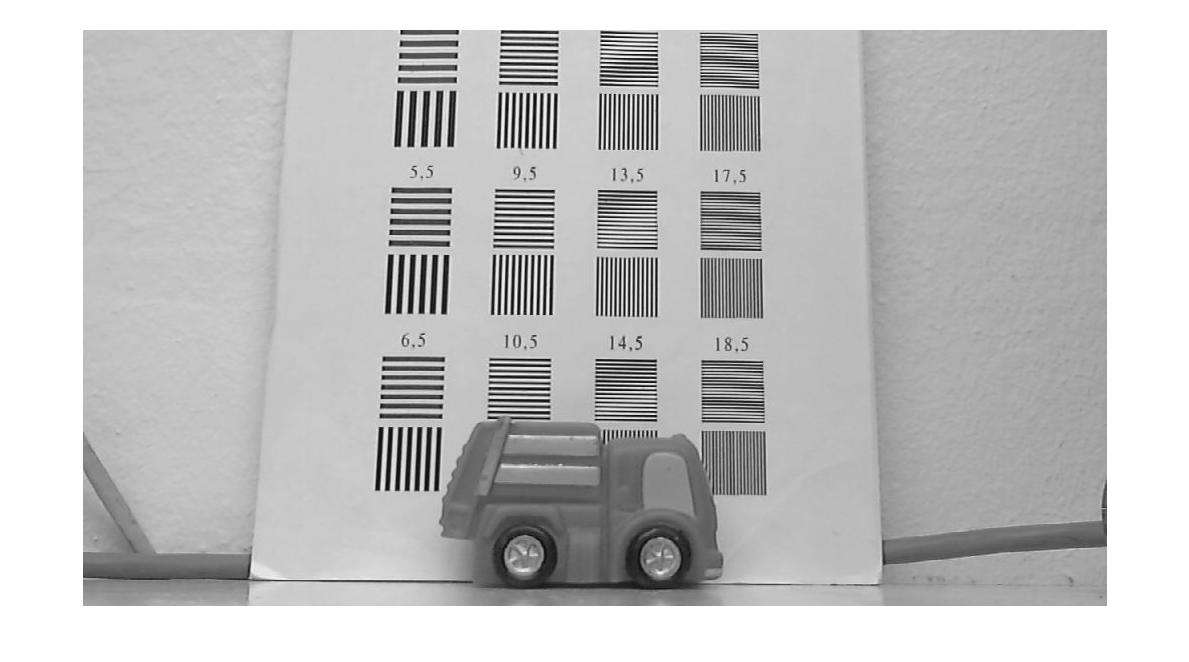
\includegraphics[width=\textwidth]{leksak1}
		\caption{}
		\label{fig:Toy1}
	\end{subfigure}
	\begin{subfigure}[b]{0.3\textwidth}
		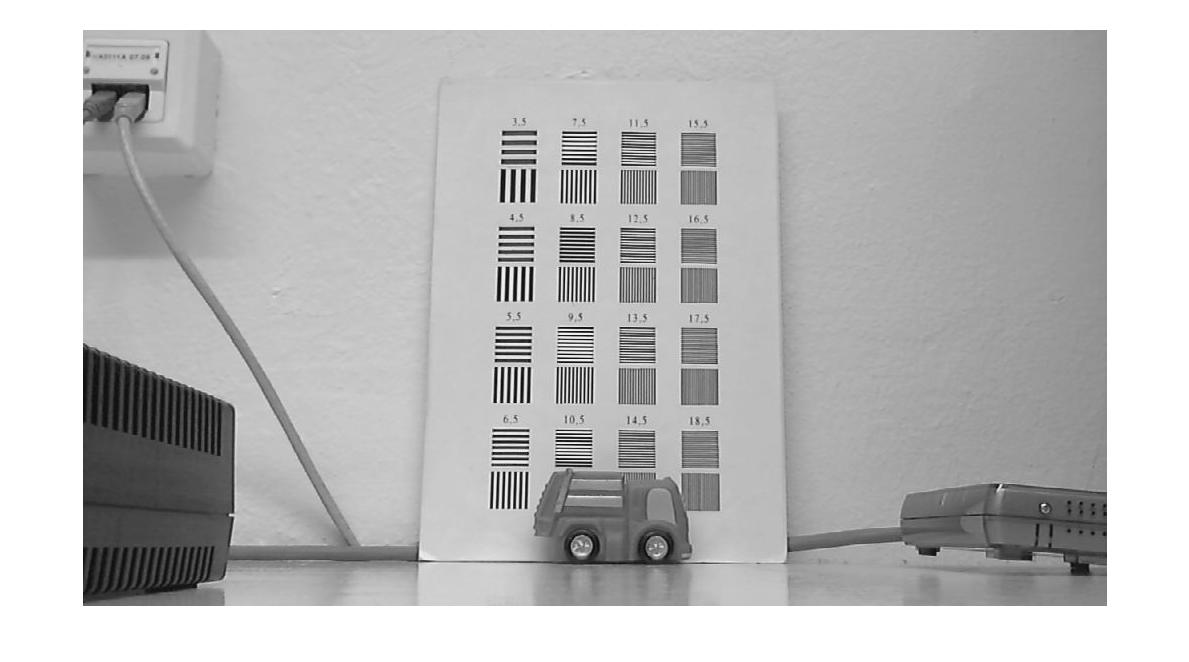
\includegraphics[width=\textwidth]{leksak2}
		\caption{}
		\label{fig:Toy2}
	\end{subfigure}
	\caption{(a) Image of test chart used to calculate how many pixels correspond to 1 cm. (b) Image used to measure distance of object and to compare the vertical and horizontal . (c) Image used to compare the resolution for different distances.}
	\label{fig:part1}
\end{figure}

\subsection{Grey scale images, image format and image information}
%\subsection{Image enhancement}
%\subsection{Colour images}
%\subsection{IR - Imaging}